\begin{figure*}[t]
\subfigure[7B (1.68$\times$$\sim$8.63$\times$)]{
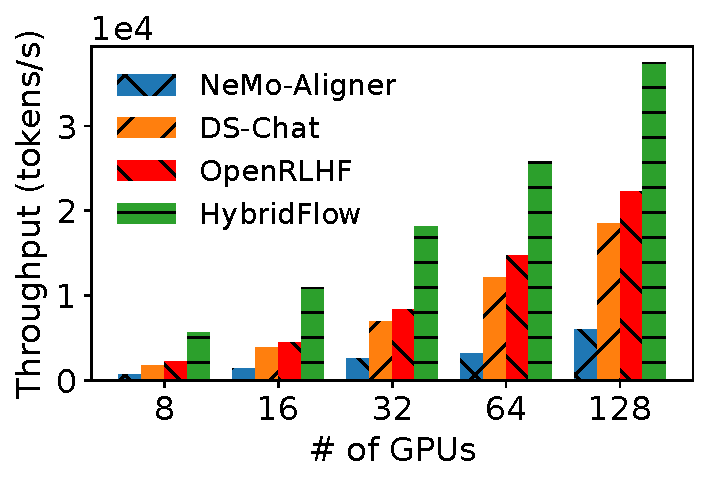
\includegraphics[width=0.25\linewidth]{figs/throughput_7B.pdf}
}
\subfigure[13B (2.70$\times$$\sim$18.96$\times$)]{
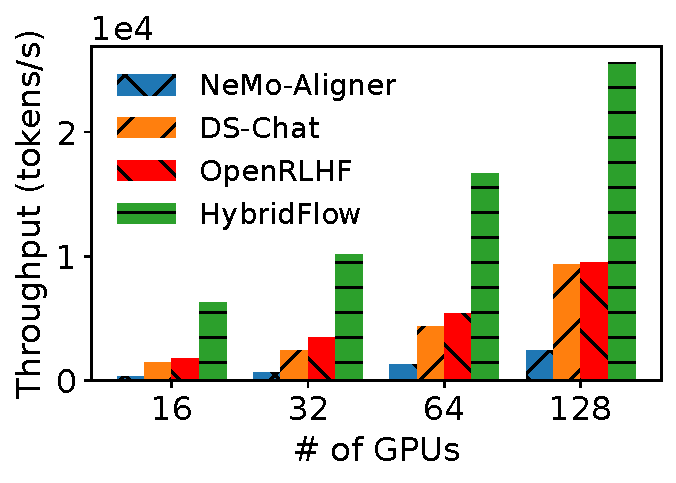
\includegraphics[width=0.24\linewidth]{figs/throughput_13B.pdf}
}
\hspace{-2mm}
\subfigure[34B (2.41$\times$$\sim$20.57$\times$)]{
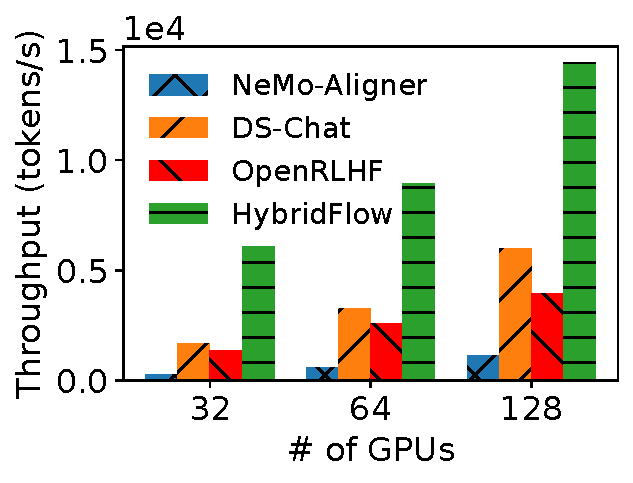
\includegraphics[width=0.23\linewidth]{figs/throughput_34B.pdf}
}
\hspace{-2mm}
\subfigure[70B (5.17$\times$$\sim$17.98$\times$)]{
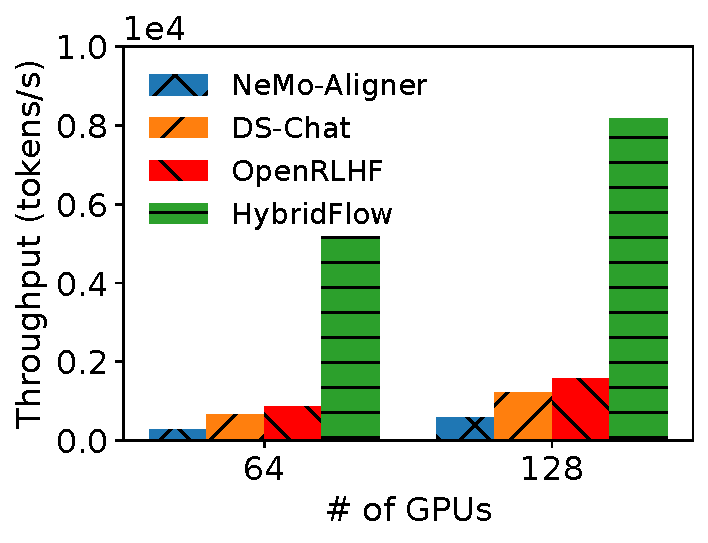
\includegraphics[width=0.22\linewidth]{figs/throughput_70B.pdf}
}
\vspace{-4mm}
\caption{PPO throughput. Numbers in parentheses are \sysname{} speedups compared with baselines.}
\vspace{-5mm}
\label{fig:train_throughput}
\end{figure*}

\begin{figure*}[t]
\vspace{-1mm}
\subfigure[7B (1.53$\times$$\sim$2.56$\times$)]{
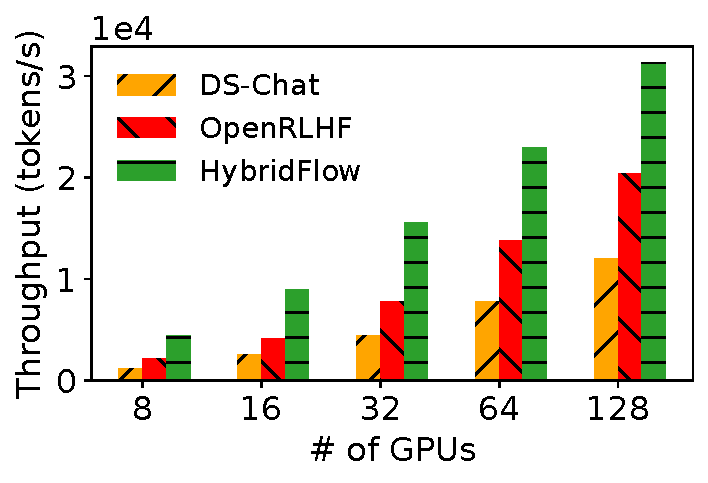
\includegraphics[width=0.25\linewidth]{figs/throughput_remax_7B.pdf}
}
\hspace{-2mm}
\subfigure[13B (2.49$\times$$\sim$3.66$\times$)]{
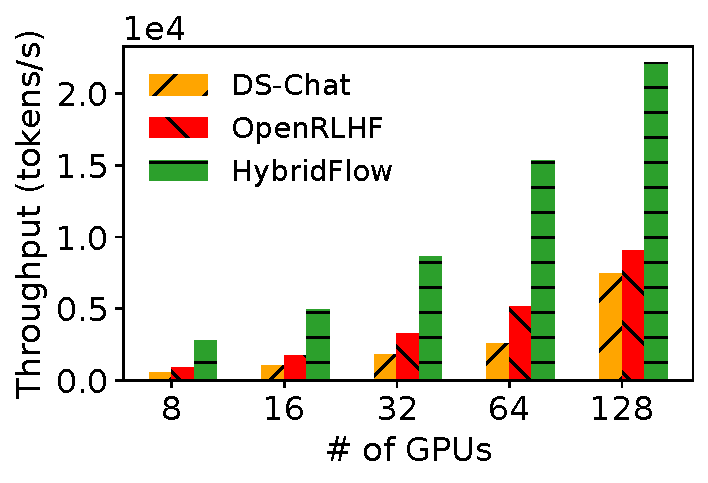
\includegraphics[width=0.25\linewidth]{figs/throughput_remax_13B.pdf}
}
\hspace{-2mm}
\subfigure[34B (2.14$\times$$\sim$4.80$\times$)]{
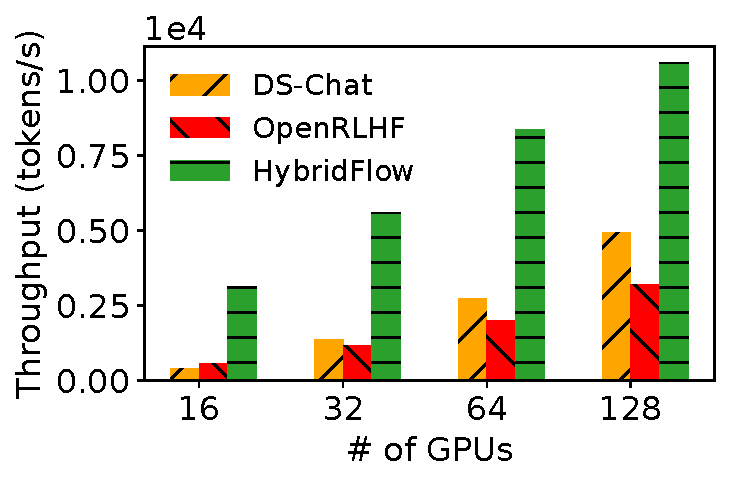
\includegraphics[width=0.25\linewidth]{figs/throughput_remax_34B.pdf}
}
\hspace{-2mm}
\subfigure[70B (6.46$\times$$\sim$9.78$\times$)]{
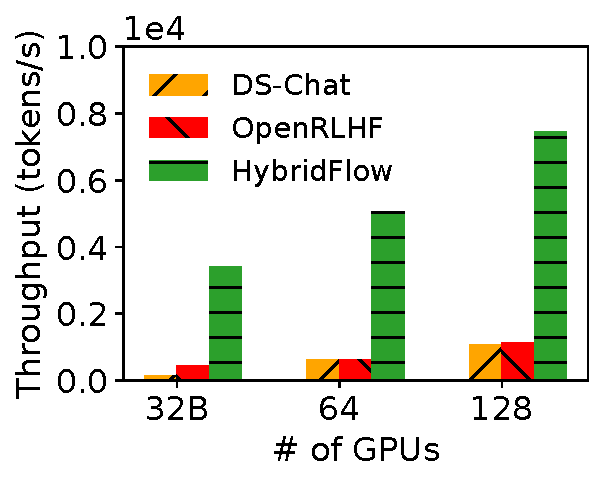
\includegraphics[width=0.21\linewidth]{figs/throughput_remax_70B.pdf}
}
\vspace{-5mm}
\caption{ReMax throughput. Numbers in parentheses are \sysname{} speedups compared with baselines}
\vspace{-5mm}
\label{fig:remax_train_throughput}
\end{figure*}

\begin{figure*}[t]
\subfigure[7B (1.71$\times$$\sim$12.87$\times$)]{
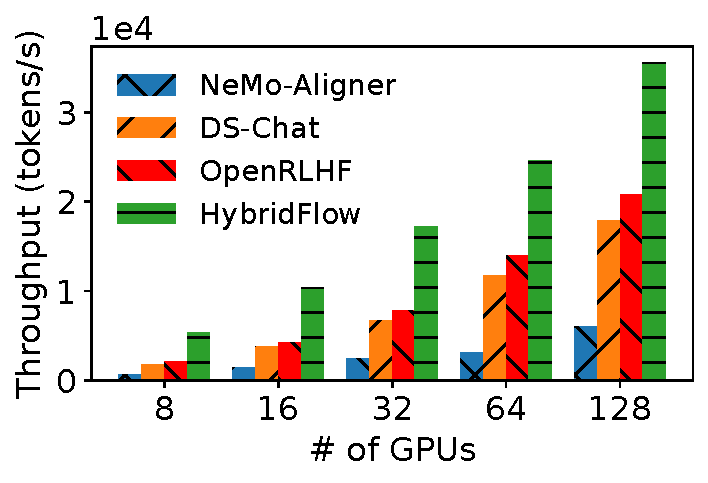
\includegraphics[width=0.25\linewidth]{figs/throughput_saferlhf_7B.pdf}
}
\subfigure[13B (2.49$\times$$\sim$18.47$\times$)]{
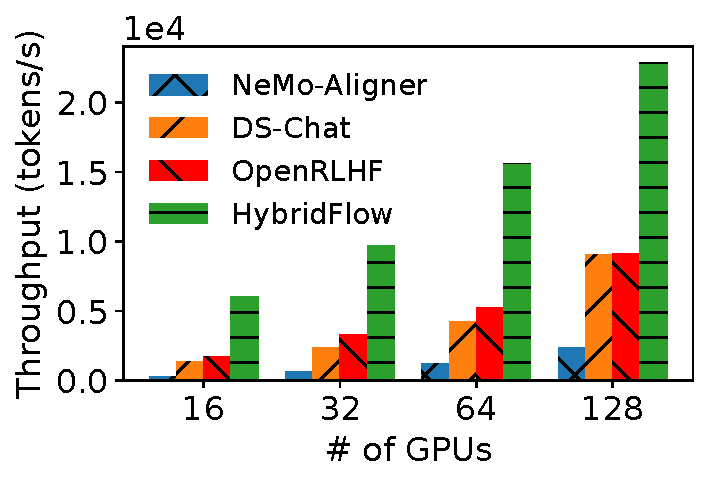
\includegraphics[width=0.25\linewidth]{figs/throughput_saferlhf_13B.pdf}
}
\hspace{-2mm}
\subfigure[34B (2.20$\times$$\sim$19.76$\times$)]{
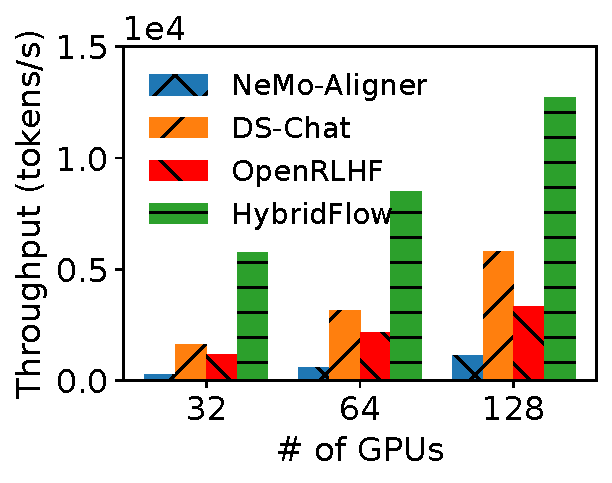
\includegraphics[width=0.22\linewidth]{figs/throughput_saferlhf_34B.pdf}
}
\hspace{-2mm}
\subfigure[70B (4.89$\times$$\sim$16.86$\times$)]{
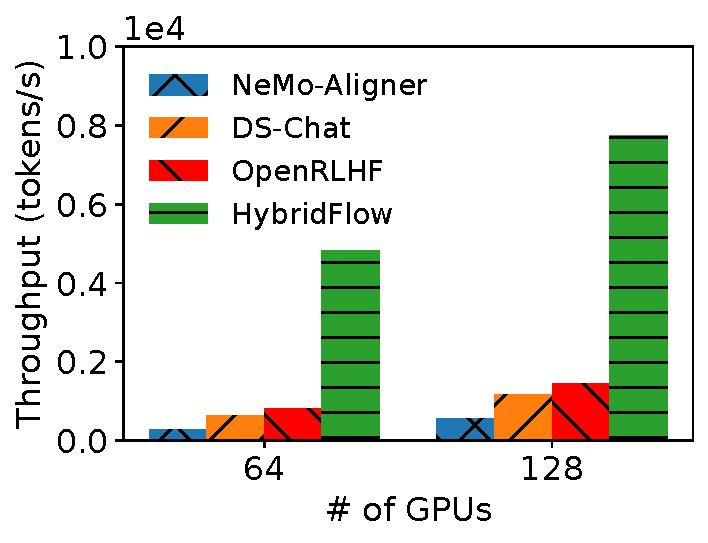
\includegraphics[width=0.22\linewidth]{figs/throughput_saferlhf_70B.pdf}
}
\vspace{-5mm}
\caption{Safe-RLHF throughput. Numbers in the parentheses are \sysname{} speedups compared with the baselines}
\vspace{-3mm}
\label{fig:safe_rlhf_train_throughput}
\end{figure*}

\section{Evaluation}

\subsection{Experimental Setup}
\textbf{Testbed.} We deploy \sysname{} on a cluster of 16 machines (128 GPUs). Each machine is equipped with 8 NVIDIA A100-80GB GPUs inter-connected with 600GB/s NVLink. The inter-machine bandwidth is 200Gbps. Our experiments use the following software versions: CUDA12.1, PyTorch 2.1.2, Megatron-core 0.6.0, NCCL 2.18.1, and vLLM 0.3.1.


\noindent\textbf{Models and RLHF algorithms.}
We %
run the RLHF dataflow (Figure~\ref{fig:rlhf_dataflow}) of PPO~\cite{schulman2017proximal}, ReMax~\cite{li2023remax} and Safe-RLHF~\cite{daiSafeRLHFSafe2023} algorithms.
PPO is one of the most popular %
algorithms for RLHF~\cite{bai2022training, ouyang2022training}, consisting of %
actor, critic, reference policy, and reward models. Each model is a Llama~\cite{touvron2023llama} model with sizes ranging from 7B to 70B. 
Safe-RLHF has an additional cost model whose architecture and size are the same as the reward model and ReMax eliminates the critic model. 
We use mixed precision for actor and critic training, i.e., BF16 for model parameters and FP32 for gradient and optimizer states, with Adam~\cite{kingma2017adam} optimizer in all experiments. 
BF16 is used in model inference and auto-regressive generation.
If not specified, the experiment results are obtained from PPO.








\noindent\textbf{Baselines.}
We compare \sysname{} with state-of-the-art RLHF systems including DeepSpeed-Chat~\cite{yao2023deepspeedchat} v0.14.0, OpenRLHF~\cite{hu23openrlhf} v0.2.5, and NeMo-Aligner~\cite{NeMoAligner} v0.2.0 (detailed in Table \ref{tab:table_with_images}). 
NeMo-Alginer doesn't support ReMax algorithm.
We do not compare \sysname{} to other frameworks such as Trlx~\cite{havrilla2023trlx}, HuggingFaceDDP~\cite{wolf2019huggingfaces}, and Collosal-Chat~\cite{CollosalChat} as they are less representative and slower than the above baselines (as reported in ~\cite{yao2023deepspeedchat}). 

We use RLHF %
throughput (tokens/sec) as the performance metric, computed by dividing the total number of tokens in prompts and responses in a global batch by one RLHF iteration time.
All reported performance %
numbers are averaged over 5 training iterations after a warm-up of 10 iterations.

\noindent\textbf{Datasets and hyperparameters.}
We perform RLHF on "Dahoas/ful-hh-rlhf" dataset~\cite{bai2022training} of HuggingFace, which is widely used for LLM alignment%
~\cite{yuan2023rrhf, santacroce2023efficient-rlhf}. %
As the baseline systems may not incorporate continuous-batching optimization~\cite{yu2022orca} during generation, for a fair comparison, we enforce the same length on all responses to be generated. In each experiment, the input prompt length and the output response length are both 1024 and the global batch size of input prompts to the actor model is 1024.
The number of PPO epochs is 1 and the number of PPO update iterations per epoch is 8, aligning with previous RLHF research~\cite{ouyang2022training, huang2024n+, xu2024dpo}.




\begin{figure*}[t]
\begin{minipage}{0.65\textwidth}
\centering
\subfigure[13B]{
    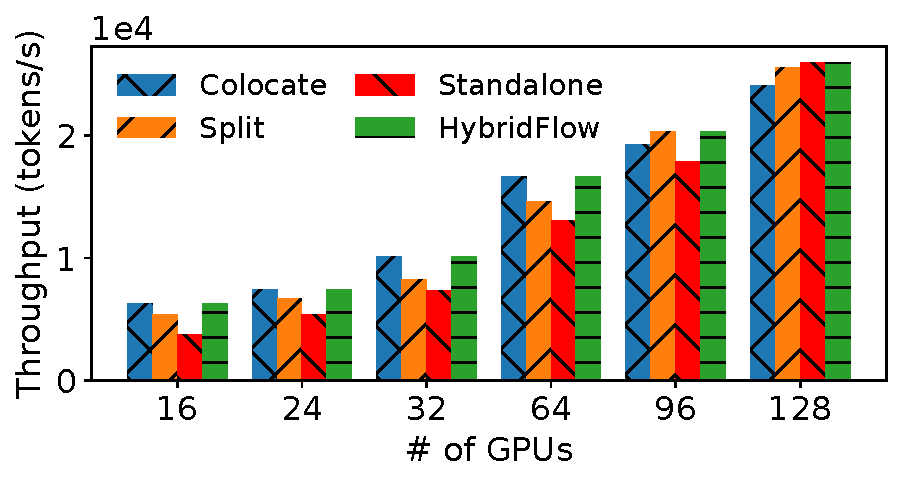
\includegraphics[width=5.5cm]{figs/placement_13B.pdf}
}
\subfigure[34B]{
    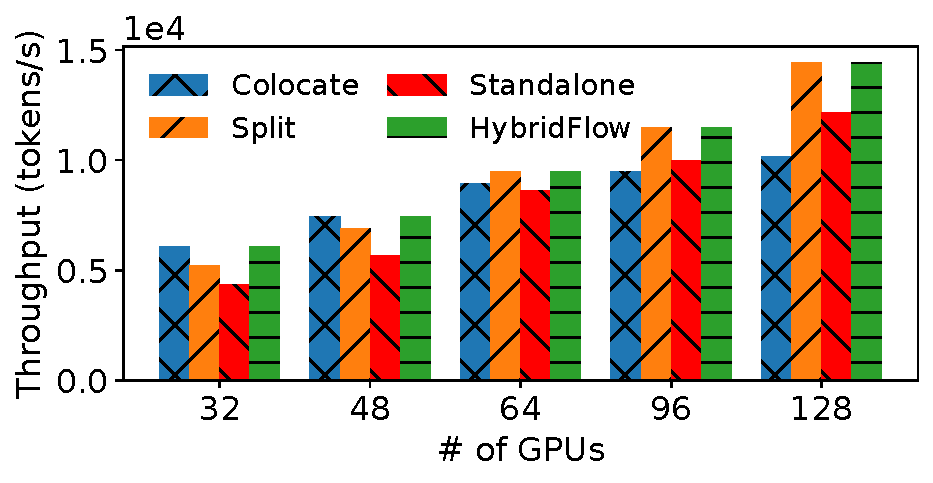
\includegraphics[width=5.5cm]{figs/placement_34B.pdf}
}
\vspace{-4mm}
\caption{Throughput of \sysname{} under different placements}
\label{fig:exp_placement}
\end{minipage}
\vspace{-3mm}
\begin{minipage}{0.33\textwidth}
    \vspace{3mm}
    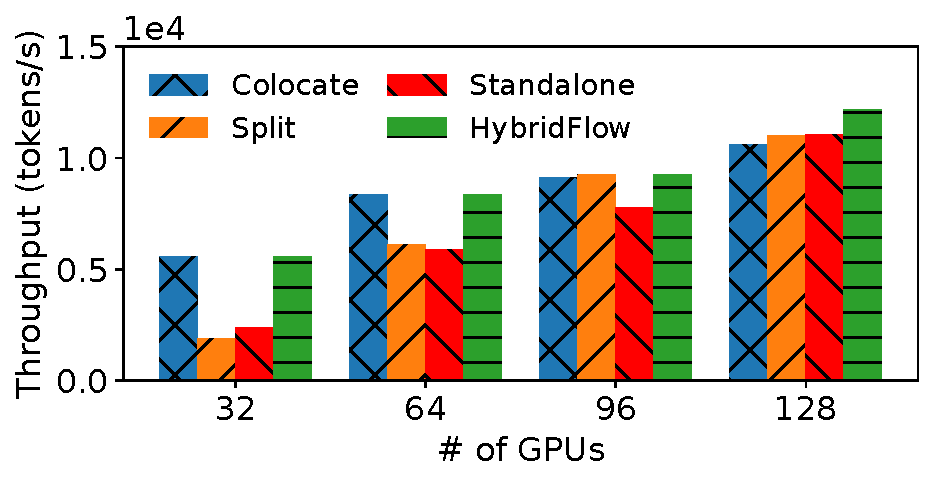
\includegraphics[width=5.5cm]{figs/placement_mix.pdf}
    \vspace{-5mm}
    \caption{Placement comparison under 13B actor and reference policy \& 70B critic and reward model.}
    \label{fig:exp_mix_placement}
\end{minipage}
\end{figure*}

\subsection{End-to-End %
performance} \label{sec:exp_e2e_train_performance}
Figures~\ref{fig:train_throughput}, \ref{fig:remax_train_throughput}, and \ref{fig:safe_rlhf_train_throughput} show RLHF throughput %
when running PPO, ReMax, and Safe-RLHF respectively. 
The actor, critic, reference, and reward models in this set of experiments are of the same size, following previous practice~\cite{bai2022training, yao2023deepspeedchat, ouyang2022training}. The number of GPUs used in experiments of different model sizes ranges from the smallest number of GPUs to run RLHF without OOM
to 128 GPUs. 
We do not enable offloading optimizer states~\cite{ren2021zerooffload} in the experiments for fair comparison.


\noindent \textbf{Overall performance.}
We observe that \sysname{} consistently outperforms the baselines across all model scales. In Figure~\ref{fig:train_throughput} for PPO, \sysname{} outperforms DeepSpeed-Chat, OpenRLHF and NeMo-Aligner by 3.67$\times$ (up to 7.84$\times$), 3.25$\times$ (up to 5.93$\times$) and 12.52$\times$ (up to 20.57$\times$), respectively. This is mainly because \sysname{} effectively executes generation, inference, and training in all RLHF stages by sharding the models with different parallelism strategies to fit various computation workloads. \sysname{} achieves the highest average speedup of 9.64$\times$ when training 70B models, 
as \sysname{} reduces the transition overhead by up to 71.2\% and 89.1\% compared to DeepSpeed-Chat and OpenRLHF, which also incurs large inter-machine communication when training with ZeRO-3.
Due to the lack of KVCache in generation engine, NeMo-Aligner's main performance bottleneck lies in the generation stage, which accounts for up to 81.2\% of its %
RLHF iteration time. %
Similar %
results can be observed in Figures ~\ref{fig:remax_train_throughput}, 
\ref{fig:safe_rlhf_train_throughput}
validating the efficiency of \sysname{} on running various RLHF algorithms.


\noindent \textbf{Scalability.} %
\sysname{} achieves at least 2.09$\times$ speedup %
on 8 GPUs. With increasing GPUs, the strong scaling efficiency of \sysname{} on various model scales is 66.8\%, computed by dividing $\frac{\mbox{throughput in largest scale}}{\mbox{throughput in smallest scale}}$ by $\frac{\mbox{max. \# of GPUs}}{\mbox{min. \# of GPUs}}$%
~\cite{amdahl1967strongscaling}, averaging over three algorithms and all model scales.
Scaling to a large number of GPUs with a fixed global batch size results in smaller local batch sizes for each worker, potentially causing GPU underutilization. Running 7B models on 128 GPUs, \sysname{} still outperforms the best baseline OpenRLHF for 1.68$\times$, 1.53$\times$, and 1.71$\times$ on PPO, ReMax, and Safe-RLHF respectively. This can be attributed to HybridFlow's ability to adapt the best placement strategies for different models and cluster sizes to minimize RLHF time. OpenRLHF performs better in a larger GPU cluster but less efficiently on smaller ones.















\begin{figure*}[t]
\vspace{-2mm}
\subfigure[7B ($T_g$=2, $P_g$=1, $T$=8,$P$=1)]{
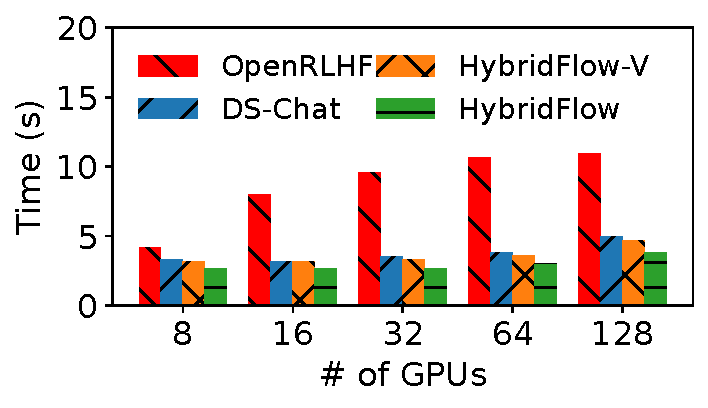
\includegraphics[width=0.25\linewidth]{figs/transit_7B.pdf}
}
\subfigure[13B ($T_g$=4, $P_g$=1, $T$=8,$P$=1)]{
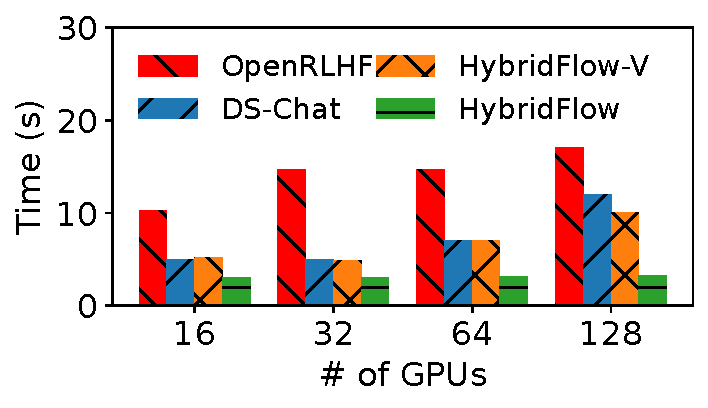
\includegraphics[width=0.25\linewidth]{figs/transit_13B.pdf}
}
\hspace{-2mm}
\subfigure[34B ($T_g$=8, $P_g$=1, $T$=8,$P$=4)]{
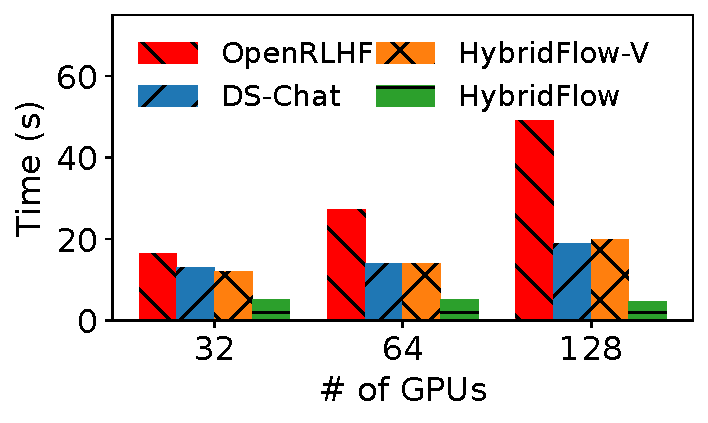
\includegraphics[width=0.23\linewidth]{figs/transit_34B.pdf}
}
\hspace{-2mm}
\subfigure[70B ($T_g$=8, $P_g$=1, $T$=8,$P$=8)]{
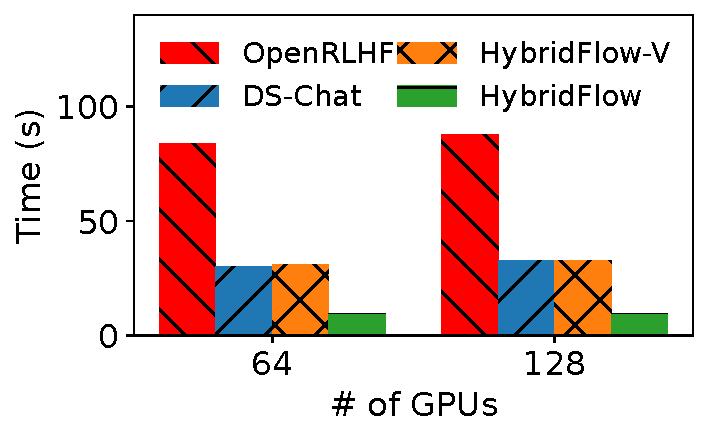
\includegraphics[width=0.225\linewidth]{figs/transit_70B.pdf}
}
\vspace{-3mm}
\caption{Transition time between actor training and generation. %
}
\vspace{-3mm}
\label{fig:exp_transit_time}
\end{figure*}

\begin{figure}[t]
    \centering
\subfigure[7B]{
    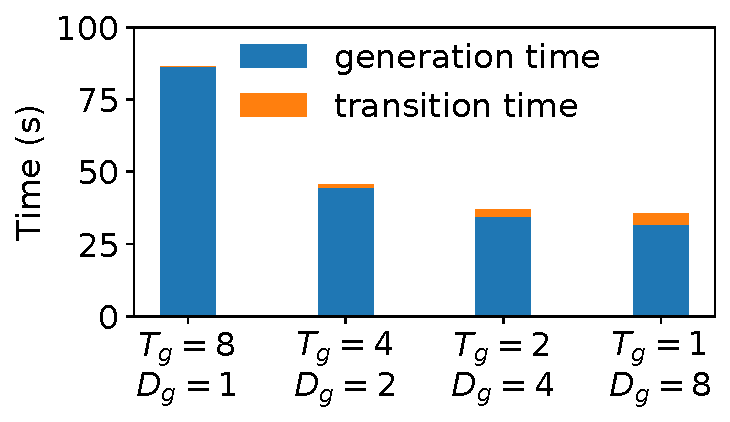
\includegraphics[width=0.48\linewidth]{figs/hybrid_breakdown_7B.pdf}
}
\hspace{-3mm}
\subfigure[13B]{
    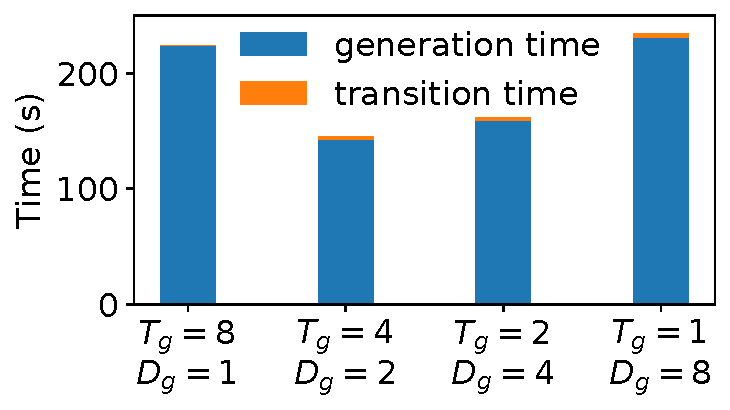
\includegraphics[width=0.48\linewidth]{figs/hybrid_breakdown_13B.pdf}
}
    \vspace{-3mm}
    \caption{%
    Time breakdown on different generation parallel sizes of the actor model on 16 GPUs. %
    }
    \vspace{-4.5mm}
    \label{fig:hybrid_breakdown}
\end{figure}


\vspace{-2mm}
\subsection{Model Placement}%
\label{sec:exp_placement}
In this experiment, we implement various model placements of the PPO algorithm in \sysname{}, under the same model and cluster settings as in Sec.~\ref{sec:exp_e2e_train_performance}: %
(i) \textit{colocate}, the placement strategy in DeepSpeed-Chat; (ii) \textit{standalone}, that in OpenRLHF and; (iii) \textit{split}, NeMo-Aligner's colocation placement (actor and reference policy on the same set of devices and critic and reward model on another); %
(iv) \textit{hybridflow}, %
the optimized placement obtained by Algorithm \ref{alg:mapping}. %


\noindent \textbf{Comparison of different model placements.}  Figure~\ref{fig:exp_placement} reveals that optimized placement of \sysname{} under different numbers of GPUs varies. From 16 to 64 GPUs, colocating all models on the same set of devices yields the best performance. 
For 96 to 128 GPUs with 34B models and 96 GPUs with 13B models, the split strategy becomes optimal. 
The split strategy divides GPUs evenly between the two sets of models, as their sizes are equal.
For 13B models on 128 GPUs, the standalone strategy achieves the highest throughput. %
In this case, \sysname{} allocates 64 GPUs for the actor, 32 for the critic, and 16 each for the reference and reward model.
In smaller clusters, computation of all models can fully utilize GPU resources; the colocate strategy ensures maximum GPU usage in different RLHF stages.
In larger clusters, RLHF throughput under colocate placement fails to scale up linearly as the batch size is fixed and the computation-to-communication ratio decreases with a larger DP size on more GPUs.
Standalone and split strategies place models on different devices with a smaller DP size for each model in larger clusters, facilitating parallel execution of different models in the same stages. %
In all cases, our Algorithm \ref{alg:mapping} produces the best placement with the highest training throughput. 






\noindent \textbf{Larger critic and reward model.} We further evaluate model placements when running PPO with a 13B actor and reference policy and 70B critic and reward models (larger critic and reward models are expected to produce better alignment~\cite{bai2022training}). Figure~\ref{fig:exp_mix_placement} shows that the colocate strategy still outperforms others by 44.8\% on average %
with up to 64 GPUs. The split strategy achieves higher throughput with 96 GPUs. When scaling to 128 GPUs, the best placement obtained by Algorithm \ref{alg:mapping} colocates actor, reference, and reward models on 64 GPUs while allocating the remaining 64 GPUs to critic.
On the same number of GPUs, actor and reference policy's computation time is much smaller than critic and reward model, and colocating the reward model with actor and reference policy reduces the GPU idle time in the experience preparation stage. 
In general, distributing actor and critic on different devices for parallel execution in the training stage leads to higher throughput in large clusters.



\subsection{%
3D-HybridEngine} \label{sec:exp_benefit_hybrid_engine}
\noindent \textbf{Transition time comparison.} 
Figure~\ref{fig:exp_transit_time} shows the transition time between actor training and generation stages on various model scales, which is the time to reshard model weights from training to generation, 
under the same settings in \textsection\ref{sec:exp_e2e_train_performance}.
OpenRLHF's transition time includes weight synchronization time between two copies of the actor model on different devices.
HybridFlow reduces the transition time by 55.2\% (11.7s) on average %
and the transition overhead by up to 89.1\% (78.2s) with 70B models, while maintaining consistent overhead across different cluster scales.
This is attributed to our new parallel grouping method for the generation stage (\textsection\ref{sec:hybrid_comm_mem}). %
In baseline methods, all model parameters must be collected during transition, necessitating layer-by-layer collections multiple times to prevent OOM.
\sysname{} enables zero memory redundancy during transition and requires only one all-gather operation per micro DP group.

\vspace{0.5mm}
\noindent \textbf{%
Transition and generation time}
We further validate the need to use different parallel sizes in actor training and generation in \sysname{}. In this experiment, all models are colocated on the same set of GPUs, and the KVCache for generation is allocated using the remaining GPU memory (i.e., best-effort allocation).
Figure~\ref{fig:hybrid_breakdown} gives the transition and generation time when running RLHF on 16 GPUs with 7B and 13B models, respectively, with training parallel groups 1-8-2 (following p-t-d convention) and varying generation TP group size $t_g$ from 1 to 8. 
The generation PP group size remains constant at $p_g$=1 and the micro DP group size $d_g$ is computed as $\frac{8}{t_g}$.
We observe that applying a smaller generation TP group size, $t_g$=2, for 7B models and $t_g$=4 for 13B models reduces the generation latency by 60.3\% and 36.4\%, respectively.
Conversely, using the same TP size as training ($t_g$=8), following the NeMo-Aligner approach, results in the largest generation latency due to GPU underutilization.
Further reducing $t_g$ fails to achieve higher speedup, as a smaller $t_g$ 
necessitates maintaining a larger KVCache per GPU.







\vspace{-1mm}
\subsection{Algorithm Runtime}
Figure~\ref{fig:exp_algo_time} shows the running time of Algorithm~\ref{alg:mapping}, 
which is significantly shorter than days of actual RLHF training. %
A linear growth of running time is exhibited, revealing good scalability of the device mapping algorithm with %
model size and cluster size. Most of the running time is spent on estimating the execution latency of each model's parallel strategies. More parallelism strategies are available for a larger model, requiring more simulations to identify the optimal one for each placement plan. %
Our caching of optimal parallelism strategies of the models to be reapplied across different placements reduces the search time for the best placement %
to at most half an hour.






\begin{figure}[t]
    \centering
    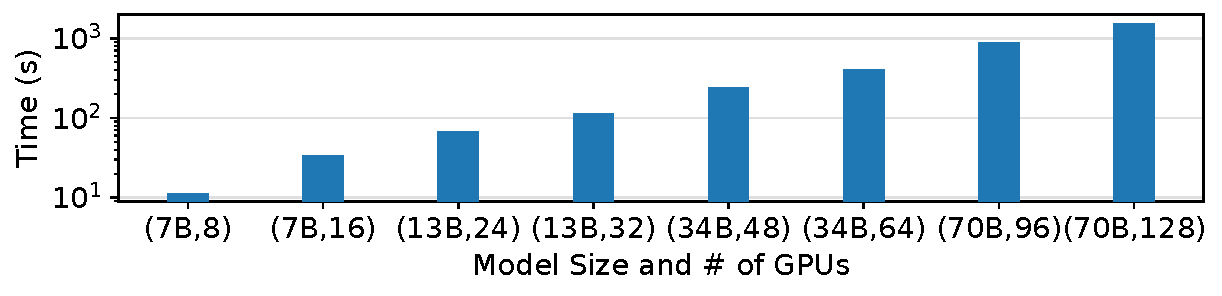
\includegraphics[width=.95\linewidth]{figs/algo_time.pdf}
    \vspace{-3mm}
    \caption{Runtime of device mapping algorithm. The model size and \# of GPUs are simultaneously scaled.}
    \label{fig:exp_algo_time}
    \vspace{-4mm}
\end{figure}
